\documentclass[12pt, a4paper, oneside]{ctexart}
\usepackage{fancyhdr}
\usepackage{amsmath, amsthm, amssymb, bm, graphicx, hyperref, mathrsfs, graphicx, float, subfigure, caption, makecell, longtable,framed}
\usepackage[dvipsnames]{xcolor}
\usepackage{listings}
\usepackage{labels}
\renewcommand{\lstlistingname}{code}
\lstset{
    language=C, % 设置语言
 basicstyle=\ttfamily, % 设置字体族
 breaklines=true, % 自动换行
 keywordstyle=\bfseries\color{NavyBlue}, % 设置关键字为粗体,颜色为 NavyBlue
 morekeywords={}, % 设置更多的关键字,用逗号分隔
 emph={self,input,output,wire,reg,posedge,negedge}, % 指定强调词,如果有多个,用逗号隔开
    emphstyle=\bfseries\color{Rhodamine}, % 强调词样式设置
    commentstyle=\itshape\color{black!50!white}, % 设置注释样式,斜体,浅灰色
    stringstyle=\bfseries\color{PineGreen!90!black}, % 设置字符串样式
    columns=flexible,
    numbers=left, % 显示行号在左边
    numbersep=2em, % 设置行号的具体位置
    numberstyle=\footnotesize, % 缩小行号
    frame=single, % 边框
    framesep=1em % 设置代码与边框的距离
}
\usepackage[left=1in, right=1in, top=1in, bottom=1in]{geometry}


\ctexset{
    % 修改 section。
    section={   
        format=\heiti\raggedright\zihao{-2} % 设置 section 标题为黑体、右对齐、小4号字
    },
    % 修改 subsection。
    subsection={   
        format=\heiti\zihao{4} % 设置 subsection 标题为黑体、5号字
    }
}


\pagestyle{fancy}
\fancyhf{}
\renewcommand{\headrulewidth}{0pt}
\fancyfoot[C]{\thepage}

\title{\textbf{8086实验报告}}
\author{张浩宇 522031910129}
\date{}

\begin{document}
    \maketitle
    \section{实验一 I/O译码}
    \subsection{读入开关状态并输出}
    \begin{figure}[!h]
        \centering
        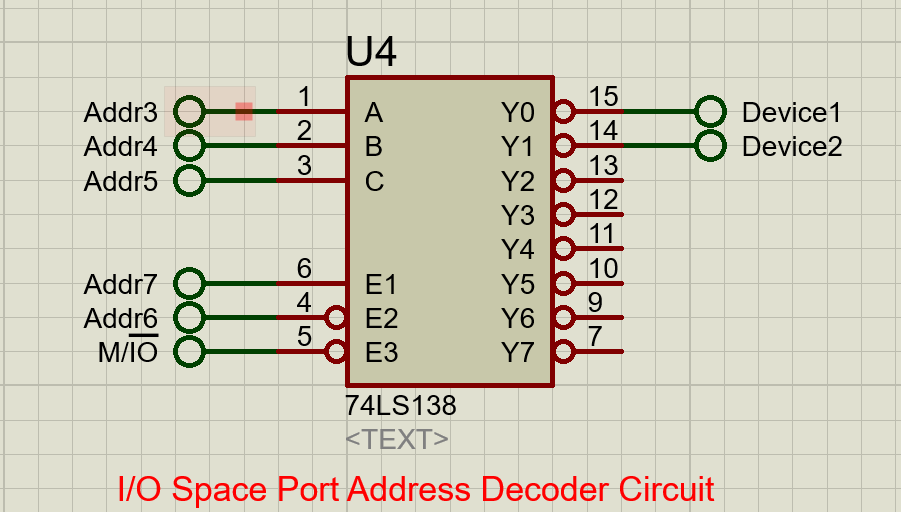
\includegraphics[width=0.8\textwidth]{img/fig1-183decoder.png}
        \label{fig:decoder}
        \caption{I/O译码电路}
    \end{figure} 
    输入口(74LS244)和输出口(74LS273)的片选端口分别为Device1和Device2,通过74LS138进行IO地址译码,如图{\ref{fig:decoder}}。
    当Device1为低电平,选中74LS244,即为输入;当Device2为低电平,选中74LS273,即为输出。根据译码器连接方式,输入端口地址80H,输出端口地址88H。
    
    因此从输入端口读入开关状态,取反输出到输出端口,即可实现开关状态的读入和输出。
    \subsection{模拟交通灯}
    如图,交通灯为6个分为2组的共阳级LED,其另一端接在74LS273输出端口,
    当对应位输出低电平时,LED亮,则每一种亮灯状态对应一个8位编码,将该编码
    从74LS273的端口地址输出就可以按照对应状态点亮LED。

    代码的运行是很快的,为了让亮灯的效果保持以便看清,需在改变LED状态后进行延时操作以保留。
    延时等待的效果可以通过循环重复多次操作实现。由于程序中需多次进行延时,可以将延时程序
    写为一个子过程,在需要时调用。

    该程序可以看作一个状态机,每个状态对应一段包括输出LED编码、延时、状态跳转的操作。从初始状态进入后,
    在不同状态之间循环,实现交通灯的模拟。

    要实现灯闪烁的效果可以通过在LED的亮和灭的状态中快速切换实现,多次切换的过程可以通过
    循环语句完成。在切换中也需要短时间的延时才能看清变化。
    \subsection{修改选片地址}
    在该电路中,74LS244和74LS273的片段端口分别为Device1和Device2,这两个端口连接在译码器的输出端,而地址总线连接在译码器的
    输入端,输入地址决定译码器的哪个输出口为低电平从而使能I/O端口芯片。因此改变Device1和Device2的在译码器上的位置就可以改变
    对应的片选地址。要改为,只需把,如图。

    要在修改选片地址后完成开关状态的写入和输出,只需将源代码中的输入和输出端口地址修改为新的地址即可。

    \subsection{实验中的问题与解决}
    在编写延时程序时,通过一层LOOP循环实现延时,但是在实际运行中发现延时时间不够长,LED状态切换过快。
    在一层LOOP循环中在添加一层由跳转语句控制的第二层循环后,延时时间变长,效果符合预期。
    \section{内存扩展和I/O空间操作}
    \subsection{8255接口操作}
    \subsubsection{8255在I/O空间的地址}

    \subsection{内存扩展}

    \section{定时器、计数器的应用}

    
\end{document}

